\documentclass[conference]{IEEEtran}
\usepackage{amsmath,amssymb,graphicx,booktabs,url,multirow,array}
% With XeTeX or LuaTeX (for example Tectonic), load an OpenType Times so bold and italic are available.
\usepackage{iftex}
\ifPDFTeX\else
\usepackage{fontspec}
\setmainfont{texgyretermes}[Extension=.otf, UprightFont=*-regular, BoldFont=*-bold, ItalicFont=*-italic, BoldItalicFont=*-bolditalic, Ligatures=TeX]
\fi
\graphicspath{{figures/}}
\title{SceneSift: Classical Cues versus Learned Features for Training-Free Video Highlight Extraction}
\author{\IEEEauthorblockN{SceneSift Project Team}
\IEEEauthorblockA{CPS 843 / CP 8307: Computer Vision}}
\begin{document}
\maketitle
\begin{abstract}
We study whether hand-built computer-vision cues, features from pretrained models, or a blend of the two best select the important moments of a video when no model is trained for the task. SceneSift cuts a video into candidate clips, measures eight kinds of evidence for each clip, and picks the highest-scoring clips that fit a length budget. Five selection methods are compared on two public benchmarks with human annotations: SumMe (25 videos), used for development, and TVSum (50 videos in 10 categories), held out and run once. On TVSum, a classical method that uses only optical-flow motion, colour histograms, edge strength, and frame differences reaches a Kendall's $\tau$ of 0.088 with annotator importance scores, close to a motion-and-audio baseline (0.097) and well above CLIP-based semantic ($-0.057$) and multimodal ($-0.009$) ranking. A blend with weights fitted on SumMe (0.028) does not improve on the classical method, and tuning the multimodal weights helps only when most of the weight moves to motion. The classical method needs less than a third of the analysis time of the multimodal one. All methods remain below human agreement (0.178) and below the best published training-free (0.135) and supervised (0.194) results.
\end{abstract}
\begin{IEEEkeywords}
video summarization, highlight detection, optical flow, colour histograms, CLIP, rank correlation
\end{IEEEkeywords}

\section{Introduction}
Long videos usually contain a few moments that viewers consider important. Video summarization and highlight extraction aim to find those moments automatically and assemble them into a short reel. What counts as important depends on the video: in a sports clip it is the action, in a how-to video it is the key steps, and in an interview it is what is said. A method built for one kind of video may fail on another.

Most recent methods train deep networks on benchmark annotations \cite{son2024csta}. That needs labelled data, and the resulting model is tied to the videos it was trained on. This project asks a narrower question that suits a setting with no training data: \emph{when nothing is trained for the task, do classical computer-vision cues, features from general-purpose pretrained models, or a blend of both agree best with human annotators?}

SceneSift is a single pipeline that applies the same steps to every video. It cuts the video into candidate clips, measures evidence for each clip, combines the evidence into one score, and selects the best clips under a length budget. The evidence is of two kinds. \emph{Classical cues} are measured directly from pixels with fundamental techniques: dense optical flow, colour histograms, Sobel gradients, and frame differencing. \emph{Learned features} come from pretrained models: CLIP image embeddings \cite{radford2021clip}, Whisper transcripts \cite{radford2023whisper}, and sentence embeddings.

The contributions are:
\begin{itemize}
\item an open pipeline with a command-line tool and a web page that produce a highlight reel, timestamps, and the evidence behind each selected clip;
\item five selection methods that share candidates, normalization, and selection, so that differences in results come from the evidence used and not from other parts of the system;
\item an evaluation on SumMe \cite{gygli2014summe} and TVSum \cite{song2015tvsum} with a strict separation between development and test data, reporting overlap F1 and rank correlation with paired tests, ablations, per-category results, and analysis cost;
\item the finding that the classical cues transfer to the held-out benchmark while request-free CLIP distinctiveness does not, and that neither a fitted blend nor tuned weights beat the classical cues there.
\end{itemize}

\section{Related Work}
\subsection{Benchmarks}
SumMe \cite{gygli2014summe} contains 25 user videos, each summarized by 15 to 18 people. TVSum \cite{song2015tvsum} contains 50 web videos in 10 categories with importance scores from 20 people for every 2-second shot. Larger collections exist: Mr.~HiSum \cite{sul2023mrhisum} derives highlight labels from audience replay statistics and VideoXum \cite{lin2023videoxum} pairs video and text summaries. We use SumMe and TVSum because they are small enough to process on one machine, have many annotators per video, and are the standard reference points for published work.

\subsection{Hand-built methods}
Early methods were built from hand-designed features. On SumMe, Gygli et al.\ \cite{gygli2014summe} segment a video into superframes and score them with hand-built interestingness features (attention, aesthetics, faces, landmarks). They report a mean F-measure of 0.234, against 0.163 for colour-histogram clustering, 0.167 for a visual-attention method, 0.143 for uniform sampling, and 0.311 for agreement between annotators. These numbers use the same protocol as this report and are the direct comparison for our SumMe results.

\subsection{Learned methods and their evaluation}
Later work trains recurrent, attention, or convolutional networks on the benchmarks themselves, usually with five-fold cross-validation. Otani et al.\ \cite{otani2019rethinking} showed that under the usual F-measure protocol, randomly generated importance scores perform about as well as published methods, because the score is dominated by how the video is segmented. They proposed measuring rank correlation between predicted and annotated importance instead. Table~\ref{tab:published} lists published rank correlations. The supervised CSTA \cite{son2024csta} is the strongest listed. Methods that train no network are the relevant comparison for this work: Pang et al.\ \cite{pang2024zeroshot} reach a Kendall's $\tau$ of 0.135 on TVSum directly from pretrained image features.
\begin{table}[t]
\caption{Published rank correlation with annotator importance scores. Supervised methods use five-fold cross-validation on the same dataset. Values for A2Summ and VASNet are as listed in \cite{son2024csta}.}
\label{tab:published}
\centering
\begin{tabular}{lcccc}
\toprule
 & \multicolumn{2}{c}{SumMe} & \multicolumn{2}{c}{TVSum} \\
Method & $\tau$ & $\rho$ & $\tau$ & $\rho$ \\
\midrule
Random \cite{otani2019rethinking} & 0.000 & 0.000 & 0.000 & 0.000 \\
DR-DSN \cite{otani2019rethinking} & -- & -- & 0.020 & 0.026 \\
dppLSTM \cite{otani2019rethinking} & -- & -- & 0.042 & 0.055 \\
Zero-shot \cite{pang2024zeroshot} & 0.096 & 0.117 & 0.135 & 0.178 \\
A2Summ & 0.108 & 0.129 & 0.137 & 0.165 \\
VASNet & 0.160 & 0.170 & 0.160 & 0.170 \\
CSTA \cite{son2024csta} & 0.246 & 0.274 & 0.194 & 0.255 \\
Human \cite{otani2019rethinking,son2024csta} & 0.205 & 0.213 & 0.177 & 0.204 \\
\bottomrule
\end{tabular}
\end{table}

\section{Method}
Fig.~\ref{fig:pipeline} shows the pipeline. Every stage is the same for every video; no category label is used at any point.
\begin{figure*}[t]
\centering
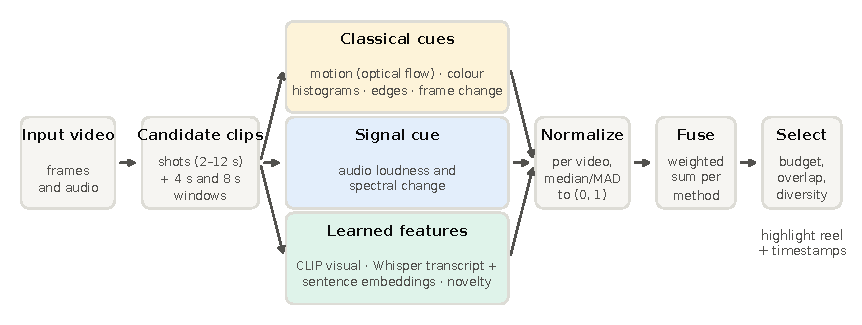
\includegraphics[width=\textwidth]{pipeline}
\caption{The SceneSift pipeline. A video is cut into candidate clips, eight kinds of evidence are measured per clip, each is normalized within the video, and a method-specific weighted sum ranks the clips for selection under a length budget.}
\label{fig:pipeline}
\end{figure*}

\subsection{Candidate clips}
A highlight can be a whole shot or a moment inside a long shot, so candidates come from two sources. Shot boundaries are detected with a content-based cut detector, and shots between 2\,s and 12\,s long become candidates. Sliding windows of 4\,s and 8\,s with 50\% overlap cover the whole video, with window edges snapped to a cut when one lies within 0.75\,s. Near-duplicate candidates are removed. Candidates in which more than half of the sampled frames are blank (black frames, fades, solid colour) are dropped, where a frame is blank when the standard deviation of its grey levels is below 6.

\subsection{Classical cues}
Four cues are measured from pixels with no pretrained model. Frames are sampled at 4 frames per second and reduced to 160-pixel-wide grey images for the dense measurements.

\emph{Motion.} Dense optical flow between consecutive samples is computed with the Farneb\"ack method. A camera pan or shake moves the whole image, so the median flow vector $\tilde{\mathbf{u}}$ is subtracted before the magnitude is averaged over the pixels $\Omega$:
\begin{equation}
m = \frac{1}{|\Omega|} \sum_{\mathbf{x} \in \Omega} \lVert \mathbf{u}(\mathbf{x}) - \tilde{\mathbf{u}} \rVert_2 .
\end{equation}
Flow between two frames on either side of a cut compares unrelated images, so those samples are discarded. A clip's motion is the mean of its samples.

\emph{Colour.} Each frame sampled at 1 frame per second is described by an HSV histogram ($8 \times 4 \times 4$ bins, square-rooted) joined to a $6 \times 6$ grey thumbnail, normalized to unit length. A clip's descriptor $\mathbf{h}_i$ is the mean over its frames. Two quantities are computed with cosine similarity: distinctiveness, $1 - \cos(\mathbf{h}_i, \bar{\mathbf{h}})$, against the mean descriptor $\bar{\mathbf{h}}$ of the whole video, and novelty, $1 - \cos(\mathbf{h}_i, \mathbf{h}_i^{-})$, against the mean descriptor $\mathbf{h}_i^{-}$ of the preceding 60\,s. The colour cue is the mean of the two after normalization.

\emph{Edges.} The mean Sobel gradient magnitude, $\frac{1}{|\Omega|}\sum_{\mathbf{x}} \sqrt{G_x^2 + G_y^2}$, measures how much fine structure a frame contains. It is low for blurred, flat, or dark frames.

\emph{Frame change.} The mean absolute grey-level difference between consecutive samples, $\frac{1}{|\Omega|}\sum_{\mathbf{x}} |I_t(\mathbf{x}) - I_{t-1}(\mathbf{x})|$, with samples across cuts discarded. Unlike optical flow it also responds to lighting changes and to camera motion.

\subsection{Signal and learned features}
\emph{Audio.} The audio track is analysed with a short-time Fourier transform. A clip's audio evidence is the mean of two normalized signals: average energy in decibels and the 90th percentile of spectral flux, which rises at sudden sounds.

\emph{Visual.} Frames sampled at 1 frame per second are embedded with OpenCLIP ViT-B/32. When the user gives a text request, a clip's visual evidence is the mean of its three highest text--image similarities. Without a request, which is the case in all experiments here, it is the clip's distinctiveness: one minus the cosine similarity between the clip's mean embedding and the whole video's.

\emph{Speech.} Whisper transcribes the audio into timestamped utterances, which are embedded with a sentence-embedding model. With a request the evidence is the highest similarity between the request and an utterance in the clip; without one it is the highest similarity to the centroid of the transcript, so utterances that are central to what the video is about score highly.

\emph{Novelty.} The mean of visual novelty (dissimilarity of the clip's CLIP embedding to the preceding 60\,s) and topic novelty (dissimilarity of an utterance to the speech of the preceding 60\,s).

\subsection{Normalization and fusion}
Raw measurements have different units and ranges, and what counts as a lot of motion depends on the video. Each feature is therefore normalized within the video by a logistic function of its robust $z$-score:
\begin{equation}
\hat{x}_i = \sigma\!\left(\frac{x_i - \operatorname{med}(x)}{1.4826 \cdot \operatorname{MAD}(x)}\right), \qquad \sigma(z) = \frac{1}{1 + e^{-z}} ,
\end{equation}
where the median and the median absolute deviation are taken over the video's candidates. The median and MAD are used instead of the mean and standard deviation so that a few extreme clips do not compress everything else. The result lies in $(0, 1)$ with 0.5 at the video's median.

The score of candidate $i$ under a method that uses the feature set $F$ is
\begin{equation}
s_i = \sum_{f \in F} \frac{w_f}{\sum_{g \in F} w_g}\, \hat{x}_{i,f} .
\end{equation}
When a kind of evidence is unavailable for a video (no audio track, no speech), it is removed from $F$ and the remaining weights are renormalized. A clip with no value for an available feature, for example a window with no speech, receives the neutral 0.5.

\subsection{Selection}
Clips are chosen greedily in order of value until the budget is filled. A candidate that overlaps an already chosen clip by more than 25\% of the shorter one is skipped. One second of context is added on each side and counted against the budget. With the diversity term on, the value of a candidate is its maximal marginal relevance,
\begin{equation}
v_i = \lambda s_i - (1 - \lambda) \max_{j \in S} \cos(\mathbf{e}_i, \mathbf{e}_j), \qquad \lambda = 0.7 ,
\end{equation}
where $S$ is the set already chosen and $\mathbf{e}$ are clip embeddings, so a clip that looks like one already chosen is penalized. The last clip is trimmed to the remaining budget, touching clips are merged, and the reel is rendered in source order.

\subsection{Compared methods}
Table~\ref{tab:methods} lists the five methods. They differ only in which features enter the weighted sum and in whether the diversity term is used. Methods A to D use fixed weights that were set by judgement before any evaluation and never tuned. The blend uses all eight features with fitted weights.
\begin{table}[t]
\caption{Compared methods. Weights are before renormalization over the features a method uses.}
\label{tab:methods}
\centering
\begin{tabular}{@{}l>{\raggedright\arraybackslash}p{4.1cm}c@{}}
\toprule
Method & Features (weight) & Diversity \\
\midrule
A: activity & motion (0.20), audio (0.15) & no \\
B: semantic & visual (0.30) & no \\
C: multimodal & visual (0.30), motion (0.20), audio (0.15), speech (0.20), novelty (0.15) & yes \\
D: classical & motion (0.20), colour (0.20), edges (0.20), frame change (0.20) & no \\
Blend & all eight, fitted on SumMe & yes \\
\bottomrule
\end{tabular}
\end{table}

\subsection{Fitting the blend}
The blend's weights are fitted on development videos by non-negative least squares. For each candidate the target is the share of the clip that annotators selected, averaged over annotators. Features (minus the neutral 0.5) and targets are centred within each video, because selection depends only on how clips rank inside their own video, and each video is scaled to count equally. Solving
\begin{equation}
\min_{\mathbf{w} \ge 0} \lVert X \mathbf{w} - \mathbf{y} \rVert_2^2
\end{equation}
and scaling $\mathbf{w}$ to sum to one gives weights in which a feature that does not help receives zero. Fitted on SumMe, the weights are audio 0.29, novelty 0.20, visual 0.19, motion 0.14, edges 0.10, frame change 0.07, and zero for speech and colour.

\subsection{Implementation}
The pipeline is written in Python with OpenCV for decoding, optical flow, and the classical cues, PySceneDetect for cuts, SciPy for audio analysis and fitting, OpenCLIP, faster-whisper, and Sentence Transformers for the learned features, and FFmpeg for rendering. One decoding pass feeds all visual measurements, and the analysis of a video is cached so that every method is scored on identical measurements. A web page built with Gradio presents the results and lets a user upload a video, choose a summary length, and inspect every method's reel and selected clips with the evidence behind each; a command-line tool also accepts a text request. The code has 72 automated tests, including an end-to-end run on a synthetic video with known events.

\section{Experimental Setup}
\subsection{Datasets}
Table~\ref{tab:datasets} summarizes the two benchmarks. SumMe videos are personal recordings such as a plane landing, cooking, and children playing. TVSum videos were collected from YouTube for ten categories: changing a vehicle tire, getting a vehicle unstuck, grooming an animal, making a sandwich, parkour, parade, flash mob gathering, bee keeping, attempting bike tricks, and dog show. Neither dataset has text requests, so all experiments test generic highlights.
\begin{table}[t]
\caption{Benchmarks.}
\label{tab:datasets}
\centering
\begin{tabular}{@{}l>{\raggedright\arraybackslash}p{2.6cm}p{2.9cm}@{}}
\toprule
 & SumMe \cite{gygli2014summe} & TVSum \cite{song2015tvsum} \\
\midrule
Videos & 25 user videos & 50 web videos, 5 in each of 10 categories \\
Total length & 67 min & 210 min \\
Annotators & 15--18 per video & 20 per video \\
Label & frames each person kept in a summary of at most 15\% & score from 1 to 5 for every 2-second shot \\
Role here & development; weights fitted & held-out test \\
\bottomrule
\end{tabular}
\end{table}

\subsection{Protocol}
SumMe is the development set. The first run of the pipeline was on SumMe, the blend's weights are fitted on it, and any choice made while building the methods could have been influenced by it. For the blend, SumMe results are therefore reported by leave-one-video-out: each video is scored with weights fitted on the other 24.

TVSum is the test set. Its annotations were converted but no method was run on it until the methods, the fixed weights, and the blend's weights were final. It was then run once. Analyses performed after that run are labelled as diagnostics.

Every summary is 15\% of the video's length, the convention for both benchmarks. An additional reference, \emph{uniform}, places evenly spaced 5-second clips to fill the same budget. It ignores the content, so it shows what a score looks like with no skill.

\subsection{Measures}
\begin{figure}[t]
\centering
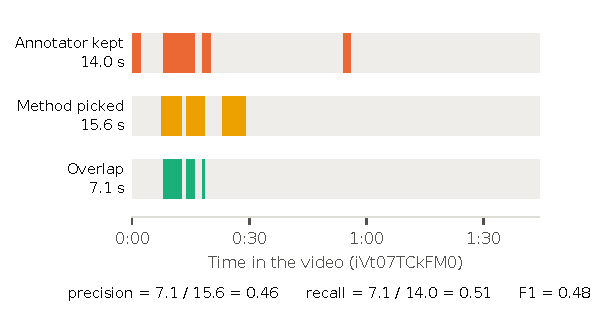
\includegraphics[width=\columnwidth]{f1}
\caption{How temporal F1 is computed against one annotator. The method's summary and the annotator's summary are aligned in time and the overlap is divided by each summary's length. The score for a video is the mean over its annotators. Video: ``Pure Fix TV: How to Wheelie'' (TVSum, CC~BY); method D.}
\label{fig:f1}
\end{figure}
\emph{Temporal F1.} Fig.~\ref{fig:f1} illustrates the measure. With $P$ the set of seconds in a method's summary and $R$ the set an annotator kept,
\begin{equation}
\text{precision} = \frac{|P \cap R|}{|P|}, \qquad \text{recall} = \frac{|P \cap R|}{|R|},
\end{equation}
\begin{equation}
F_1 = \frac{2 \cdot \text{precision} \cdot \text{recall}}{\text{precision} + \text{recall}} .
\end{equation}
Precision is the share of the method's summary that the annotator also wanted; recall is the share of the annotator's summary that the method found. F1 is computed against each annotator separately and averaged, which is the SumMe protocol \cite{gygli2014summe}. On SumMe each annotator's summary is given. On TVSum each annotator's reference summary is built from their scores: their highest-rated shots up to 15\% of the video, with ties broken in favour of shots whose neighbours are rated higher and then earlier shots.

\emph{Rank correlation.} F1 only looks at the clips that were selected. Rank correlation asks whether a method orders all moments of the video the way people do. The candidate scores are turned into a curve over time, where each time bin receives the mean score of the candidates that contain it. Kendall's $\tau$ and Spearman's $\rho$ are computed between that curve and each annotator's scores and averaged over annotators. Kendall's $\tau$ compares every pair of bins: it is the number of pairs ordered the same way by both minus the number ordered oppositely, divided by the number of pairs, with a correction for ties. It is 1 for identical orderings, $-1$ for reversed orderings, and 0 on average for random scores. On TVSum the annotator scores are the ratings of the 2-second shots. On SumMe they are the share of each second that the annotator kept. Following \cite{otani2019rethinking}, rank correlation is the main measure on TVSum.

\emph{Other measures.} Event coverage is the share of an annotator's intervals that have at least half their duration in the summary. Redundancy is the mean pairwise cosine similarity between the CLIP embeddings of the selected clips. Analysis cost is the processing time of the stages a method needs, in seconds per minute of video, excluding model loading.

\emph{Human agreement.} As a ceiling, the same measures are computed between annotators: the mean pairwise F1 and the mean pairwise Kendall's $\tau$.

\emph{Uncertainty.} Differences between two methods are computed per video and reported with a 95\% bootstrap interval of the mean difference (10{,}000 resamples of videos) and a Wilcoxon signed-rank $p$-value. The $p$-values are not corrected for multiple comparisons and should be read as descriptive.

\subsection{Hypotheses}
Four hypotheses were stated before the experiments.
\begin{itemize}
\item H1: the multimodal method C scores above the activity baseline A.
\item H2: C scores above the semantic baseline B.
\item H3: the diversity term reduces repeated content without reducing coverage of important events.
\item H4: the classical method D scores above evenly spaced clips, and the blend scores above both D and C.
\end{itemize}

\subsection{Environment}
All runs used a 16-core AMD Ryzen Threadripper PRO 5955WX with no GPU. The models were OpenCLIP ViT-B/32 (LAION-2B weights), Whisper \emph{base}, and all-MiniLM-L6-v2.

\section{Results}
\begin{figure*}[t]
\centering
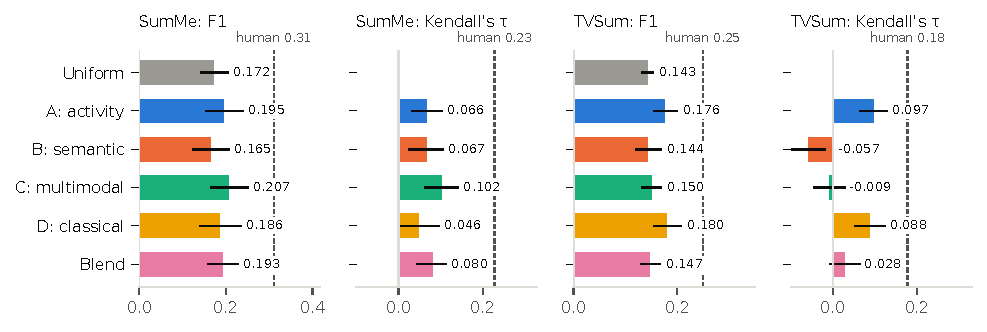
\includegraphics[width=\textwidth]{results}
\caption{Mean F1 and Kendall's $\tau$ per method with 95\% bootstrap intervals over videos. The dashed line is the agreement between human annotators. On SumMe the blend is shown by leave-one-video-out. The uniform reference has no scores and therefore no $\tau$.}
\label{fig:results}
\end{figure*}
\begin{table}[t]
\caption{Main results: mean over videos. SumMe: 25 videos (development). TVSum: 50 videos (held out). Blend on SumMe is leave-one-video-out, with the in-sample value in parentheses.}
\label{tab:results}
\centering
\setlength{\tabcolsep}{3.2pt}
\begin{tabular}{@{}lcccccc@{}}
\toprule
 & \multicolumn{3}{c}{SumMe} & \multicolumn{3}{c}{TVSum} \\
Method & F1 & $\tau$ & $\rho$ & F1 & $\tau$ & $\rho$ \\
\midrule
Uniform & 0.172 & -- & -- & 0.143 & -- & -- \\
A: activity & 0.195 & 0.066 & 0.082 & 0.176 & \textbf{0.097} & \textbf{0.127} \\
B: semantic & 0.165 & 0.067 & 0.084 & 0.144 & $-0.057$ & $-0.076$ \\
C: multimodal & \textbf{0.207} & \textbf{0.102} & \textbf{0.127} & 0.150 & $-0.009$ & $-0.011$ \\
D: classical & 0.186 & 0.046 & 0.058 & \textbf{0.180} & 0.088 & 0.114 \\
Blend & 0.193 & 0.080 & 0.099 & 0.147 & 0.028 & 0.036 \\
 & (0.212) & (0.103) & (0.128) & & & \\
\midrule
Human & 0.311 & 0.229 & -- & 0.250 & 0.178 & -- \\
\bottomrule
\end{tabular}
\end{table}
Table~\ref{tab:results} and Fig.~\ref{fig:results} give the main results.

\subsection{SumMe (development)}
The multimodal method C has the highest F1 (0.207) and $\tau$ (0.102) among the fixed-weight methods. Table~\ref{tab:paired} shows which differences the 25 videos can distinguish. C exceeds the semantic baseline B on both measures and exceeds the classical method D on rank correlation. C is not distinguishable from the activity baseline A, and no method is distinguishable from evenly spaced clips on F1: the interval for C minus uniform is $-0.012$ to $+0.086$. D is above uniform on average (0.186 against 0.172) but the interval spans zero.

Fitting the blend did not help on SumMe. On the videos it was fitted on it reaches 0.212, level with C, but on held-out videos it reaches 0.193 F1 and 0.080 $\tau$, both below the untuned C.

No method reaches the 0.234 that Gygli et al.\ report for hand-built features under the same protocol, although A, C, and D are above the simple baselines they report (0.143 to 0.167). On rank correlation, C's 0.102 is level with the published training-free result on SumMe (0.096, Table~\ref{tab:published}).

\subsection{TVSum (held out)}
On TVSum the ordering reverses. The two methods that use no CLIP features, A and D, have the highest rank correlation (0.097 and 0.088) and the highest F1 (0.176 and 0.180). The two that depend on CLIP distinctiveness are at or below chance: B has $\tau = -0.057$ and C has $-0.009$.

The paired comparisons in Table~\ref{tab:paired} are clear. D exceeds C by 0.096 in $\tau$ (interval 0.059 to 0.134) and is better on 40 of the 50 videos; D exceeds B by 0.145 and is better on 42. A and D are not distinguishable from each other. D is the only method distinguishably above evenly spaced clips on F1 ($+0.037$, interval 0.009 to 0.068). The blend fitted on SumMe is above C by 0.037 but below D by 0.059 and below A by 0.069.
\begin{table}[t]
\caption{Paired differences across videos: mean difference, 95\% bootstrap interval, number of videos where the first method is better, and Wilcoxon $p$. Blend rows on SumMe use the in-sample blend.}
\label{tab:paired}
\centering
\setlength{\tabcolsep}{3pt}
\begin{tabular}{@{}llcccc@{}}
\toprule
Comparison & & Diff. & Interval & Wins & $p$ \\
\midrule
\multicolumn{6}{@{}l}{\emph{SumMe (25 videos)}} \\
C $-$ B & F1 & $+0.042$ & $+0.011, +0.079$ & 17 & 0.037 \\
C $-$ A & F1 & $+0.012$ & $-0.016, +0.053$ & 12 & 0.98 \\
C $-$ D & F1 & $+0.021$ & $-0.010, +0.057$ & 12 & 0.48 \\
C $-$ uniform & F1 & $+0.034$ & $-0.012, +0.086$ & 16 & 0.22 \\
D $-$ uniform & F1 & $+0.013$ & $-0.040, +0.072$ & 11 & 0.90 \\
Blend $-$ C & F1 & $+0.005$ & $-0.046, +0.052$ & 13 & 0.47 \\
C $-$ B & $\tau$ & $+0.035$ & $+0.012, +0.059$ & 19 & 0.008 \\
C $-$ A & $\tau$ & $+0.037$ & $-0.003, +0.075$ & 17 & 0.13 \\
C $-$ D & $\tau$ & $+0.056$ & $+0.015, +0.096$ & 18 & 0.013 \\
D $-$ A & $\tau$ & $-0.019$ & $-0.053, +0.015$ & 12 & 0.30 \\
\midrule
\multicolumn{6}{@{}l}{\emph{TVSum (50 videos)}} \\
D $-$ B & $\tau$ & $+0.145$ & $+0.097, +0.195$ & 42 & $<0.001$ \\
D $-$ C & $\tau$ & $+0.096$ & $+0.059, +0.134$ & 40 & $<0.001$ \\
D $-$ A & $\tau$ & $-0.009$ & $-0.033, +0.015$ & 23 & 0.61 \\
A $-$ C & $\tau$ & $+0.105$ & $+0.067, +0.144$ & 40 & $<0.001$ \\
C $-$ B & $\tau$ & $+0.049$ & $+0.027, +0.072$ & 32 & $<0.001$ \\
Blend $-$ C & $\tau$ & $+0.037$ & $+0.014, +0.059$ & 35 & 0.002 \\
Blend $-$ D & $\tau$ & $-0.059$ & $-0.093, -0.027$ & 15 & $<0.001$ \\
Blend $-$ A & $\tau$ & $-0.069$ & $-0.100, -0.038$ & 14 & $<0.001$ \\
D $-$ uniform & F1 & $+0.037$ & $+0.009, +0.068$ & 28 & 0.046 \\
D $-$ C & F1 & $+0.030$ & $+0.005, +0.059$ & 31 & 0.053 \\
A $-$ C & F1 & $+0.026$ & $+0.005, +0.049$ & 30 & 0.035 \\
C $-$ uniform & F1 & $+0.007$ & $-0.011, +0.027$ & 23 & 0.87 \\
Blend $-$ uniform & F1 & $+0.004$ & $-0.015, +0.025$ & 24 & 0.95 \\
\bottomrule
\end{tabular}
\end{table}

\subsection{Other measures and cost}
Table~\ref{tab:secondary} reports precision, recall, event coverage, redundancy, and analysis cost. Precision and recall are close for every method because the summary and the references have similar lengths. Event coverage follows F1.

The methods that use CLIP features select less repetitive clips: on TVSum the redundancy of B and C is about 0.55 against 0.76 to 0.78 for A and D. This is expected, since B and C reward clips that look unlike the rest of the video, but on TVSum that variety did not coincide with what annotators rated as important.

A and D cost 1.2 to 1.8 seconds of analysis per minute of video. C and the blend cost 4.1 to 4.4 seconds, because they add CLIP inference and speech transcription. D is therefore under a third of the cost of C on TVSum.
\begin{table}[t]
\caption{Other measures: precision (P), recall (R), event coverage (Cov.), redundancy (Red.), and analysis seconds per minute of video. SumMe blend values are in-sample.}
\label{tab:secondary}
\centering
\setlength{\tabcolsep}{3.5pt}
\begin{tabular}{@{}lccccc@{}}
\toprule
Method & P & R & Cov. & Red. & s/min \\
\midrule
\multicolumn{6}{@{}l}{\emph{SumMe}} \\
Uniform & 0.163 & 0.186 & 0.172 & -- & 0 \\
A: activity & 0.185 & 0.211 & 0.204 & 0.841 & 1.7 \\
B: semantic & 0.160 & 0.174 & 0.181 & 0.763 & 2.3 \\
C: multimodal & 0.198 & 0.221 & 0.215 & 0.769 & 4.1 \\
D: classical & 0.178 & 0.198 & 0.193 & 0.856 & 1.8 \\
Blend & 0.201 & 0.229 & 0.233 & 0.787 & 4.3 \\
\midrule
\multicolumn{6}{@{}l}{\emph{TVSum}} \\
Uniform & 0.140 & 0.146 & 0.138 & -- & 0 \\
A: activity & 0.173 & 0.180 & 0.201 & 0.779 & 1.2 \\
B: semantic & 0.142 & 0.146 & 0.160 & 0.540 & 2.0 \\
C: multimodal & 0.148 & 0.152 & 0.167 & 0.559 & 4.3 \\
D: classical & 0.178 & 0.183 & 0.193 & 0.762 & 1.3 \\
Blend & 0.145 & 0.150 & 0.169 & 0.597 & 4.4 \\
\bottomrule
\end{tabular}
\end{table}

\subsection{Ablations}
\begin{figure}[t]
\centering
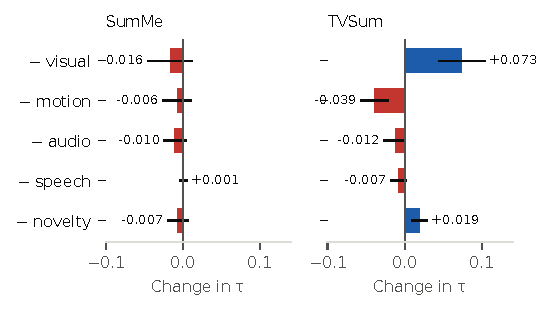
\includegraphics[width=\columnwidth]{ablation}
\caption{Change in the multimodal method's Kendall's $\tau$ when one feature is removed, with 95\% bootstrap intervals. Blue: removing the feature helps. Red: removing it hurts.}
\label{fig:ablation}
\end{figure}
Table~\ref{tab:ablation} and Fig.~\ref{fig:ablation} show C with one feature removed at a time, and without the diversity term. On SumMe every removal changes the scores by amounts within noise; removing audio costs the most F1 (0.207 to 0.186). On TVSum the picture is sharper. Removing the visual feature \emph{raises} $\tau$ from $-0.009$ to 0.065, and removing novelty raises it slightly. Removing motion lowers it the most, to $-0.047$. The visual feature is thus the cause of C's failure on TVSum, and motion is what holds C up.

The diversity term lowers redundancy on both datasets (0.769 against 0.806 on SumMe, 0.559 against 0.655 on TVSum) and changes neither F1, coverage, nor $\tau$ by a measurable amount.
\begin{table}[t]
\caption{Ablations of the multimodal method C.}
\label{tab:ablation}
\centering
\setlength{\tabcolsep}{4pt}
\begin{tabular}{@{}lcccccc@{}}
\toprule
 & \multicolumn{3}{c}{SumMe} & \multicolumn{3}{c}{TVSum} \\
Variant & F1 & $\tau$ & Red. & F1 & $\tau$ & Red. \\
\midrule
C, full & 0.207 & 0.102 & 0.769 & 0.150 & $-0.009$ & 0.559 \\
$-$ visual & 0.203 & 0.087 & 0.810 & 0.152 & 0.065 & 0.626 \\
$-$ motion & 0.201 & 0.096 & 0.742 & 0.145 & $-0.047$ & 0.536 \\
$-$ audio & 0.186 & 0.092 & 0.770 & 0.151 & $-0.021$ & 0.549 \\
$-$ speech & 0.198 & 0.103 & 0.763 & 0.149 & $-0.016$ & 0.565 \\
$-$ novelty & 0.203 & 0.096 & 0.776 & 0.152 & 0.010 & 0.579 \\
$-$ diversity & 0.204 & 0.102 & 0.806 & 0.150 & $-0.009$ & 0.655 \\
\bottomrule
\end{tabular}
\end{table}

\subsection{Results by category}
\begin{figure}[t]
\centering
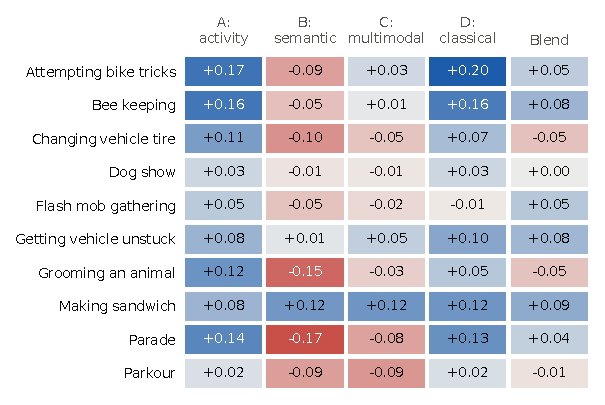
\includegraphics[width=\columnwidth]{categories}
\caption{Mean Kendall's $\tau$ on TVSum by category (five videos each). Blue: agreement with annotators. Red: disagreement.}
\label{fig:categories}
\end{figure}
Fig.~\ref{fig:categories} breaks the TVSum rank correlation down by category. A and D are positive in nearly every category and strongest where the important moments involve visible action: bike tricks (0.17 and 0.20), bee keeping (0.16 and 0.16), and parades (0.14 and 0.13). They are weakest for dog shows and parkour, where there is motion throughout and motion alone does not single out the important parts. B is negative in eight of the ten categories. The one category where the CLIP-based methods do as well as the others is making a sandwich (0.12 for B, C, and D), where the important steps look different from the rest of the video. With five videos per category these patterns are descriptive only.

\subsection{Tuning the multimodal weights}
After the held-out run we asked whether different weights for the same five features would rescue C. Table~\ref{tab:tuning} gives the results; the TVSum columns are diagnostics, not held-out results.

Two ways of choosing weights on SumMe were tried: the least-squares fit of Section~III, and a grid search over all weight combinations in steps of 0.1 (1{,}001 combinations) for the best mean F1. The grid search finds weights that score 0.228 on the videos it searched over, but on held-out SumMe videos it scores 0.180, below the untuned 0.207: with 25 videos the search fits noise. Both sets of SumMe-chosen weights raise TVSum $\tau$ only from $-0.009$ to about 0.014 (interval of the gain for the grid search: $+0.009$ to $+0.037$), still far below D.

Fitting within TVSum by leave-one-video-out, the protocol supervised methods use, does bring C level with D (0.086). It does so by placing two thirds of the weight on motion (motion 0.67, visual 0.12, audio 0.11, speech 0.10, novelty 0). The same cross-validated fit gives 0.082 for the blend and 0.090 for D. No linear weighting of these features exceeded about 0.09 on TVSum.
\begin{table}[t]
\caption{Tuning the weights of the multimodal method C. ``Held out'' on SumMe is leave-one-video-out. TVSum values were computed after the held-out run and are diagnostics.}
\label{tab:tuning}
\centering
\setlength{\tabcolsep}{3.5pt}
\begin{tabular}{@{}p{2.7cm}cccc@{}}
\toprule
 & \multicolumn{2}{c}{SumMe F1} & \multicolumn{2}{c}{TVSum} \\
Weights & all & held out & $\tau$ & F1 \\
\midrule
Untuned & 0.207 & -- & $-0.009$ & 0.150 \\
Least squares on SumMe & 0.197 & 0.192 & 0.013 & 0.146 \\
Grid search on SumMe & 0.228 & 0.180 & 0.014 & 0.143 \\
Least squares within TVSum (cross-validated) & -- & -- & 0.086 & 0.178 \\
\midrule
D: classical, untuned & 0.186 & -- & 0.088 & 0.180 \\
\bottomrule
\end{tabular}
\end{table}

\subsection{Comparison with published results}
On TVSum, D (0.088) and A (0.097) are above the trained dppLSTM (0.042) and DR-DSN (0.020) as measured in \cite{otani2019rethinking}, below the training-free method of \cite{pang2024zeroshot} (0.135), and well below supervised methods such as VASNet (0.160) and CSTA (0.194). The pairwise human $\tau$ measured here on TVSum (0.178) matches the published 0.177, which indicates that the measure is computed in the standard way. On SumMe, C's $\tau$ of 0.102 is level with the training-free 0.096, and no method reaches the hand-built F1 of 0.234 \cite{gygli2014summe}.

\subsection{A worked example}
\begin{figure*}[t]
\centering
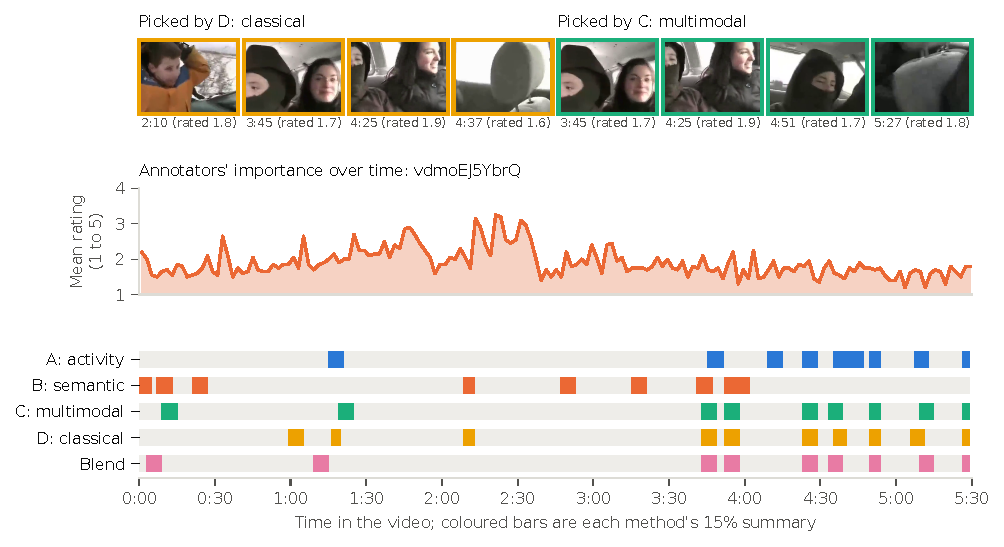
\includegraphics[width=\textwidth]{example}
\caption{One TVSum video, chosen as the video with the median difference between D and C so that it is typical and not hand-picked. Top: frames from the four highest-scoring clips of D and of C, with the annotators' mean rating of that moment. Middle: the mean rating of every 2-second shot. Bottom: each method's 15\% summary. Video: ``\#453 girl gets van stuck in the back fourty [Davidsfarm]'' (TVSum, CC~BY).}
\label{fig:example}
\end{figure*}
Fig.~\ref{fig:example} shows one TVSum video in detail. The annotators' ratings are highest between 1:30 and 2:40 and low in the last two minutes. All five methods place most of their summary after 3:40, in the low-rated part, which is why their scores on this video are near zero (D $+0.03$, C $-0.05$). D and A place one or two clips in the first half; D's clip at 2:10 falls in the highest-rated stretch. The example shows both the difference between the methods and how far all of them are from the annotators: what people rated as important here is the progress of the story, which none of the measured signals captures.

\section{Discussion}
\subsection{Outcome of the hypotheses}
Table~\ref{tab:hypotheses} summarizes the outcome of each hypothesis.
\begin{table}[t]
\caption{Outcome of the hypotheses.}
\label{tab:hypotheses}
\centering
\begin{tabular}{@{}p{2.5cm}p{2.6cm}p{2.6cm}@{}}
\toprule
Hypothesis & SumMe & TVSum (held out) \\
\midrule
H1: C above A & Not distinguishable & Not supported; A is clearly above C \\
H2: C above B & Supported & Supported, but B is below chance \\
H3: diversity lowers redundancy, keeps coverage & Supported & Supported \\
H4a: D above uniform & Not distinguishable & Supported on F1 \\
H4b: blend above D and C & Not supported & Above C, below D \\
\bottomrule
\end{tabular}
\end{table}

\subsection{Why the classical cues transferred and CLIP distinctiveness did not}
Without a text request, the visual feature scores how unlike the rest of the video a clip looks. On SumMe's unedited recordings this is mildly useful: an unusual view often is the event the video was recorded for. On TVSum's edited web videos it is negatively related to what annotators rated as important. A plausible reason is that the segments that look least like the rest of an edited video are title cards, credits, cutaways, and transitions, which annotators rate low. The same weakness appeared in informal checks on other footage, where logo cards, a watermarked clip, and the one colour shot in a black-and-white reel were selected. The category results agree with this reading: the CLIP-based methods do well only for sandwich making, where the important steps do look different.

Motion and frame change, in contrast, mark moments where something is happening, and that carried over from one dataset to the other. They are also normalized within each video, which removes differences in resolution and camera work between videos.

This result concerns request-free scoring only. With a request, the visual feature measures similarity between the frames and the text, which is what CLIP was trained for. Neither benchmark contains requests, so that mode is available in the command-line tool but not measured.

\subsection{Why the blend and the tuning did not help}
The least-squares fit gave weight to what predicts annotator selections on SumMe: audio, novelty, and visual distinctiveness. Those preferences did not hold on TVSum, where motion and frame change predict importance. Twenty-five development videos are too few to fit eight weights reliably, as the gap between in-sample and held-out SumMe scores shows, and they are a different kind of video from the test set. The cross-validated fit within TVSum shows that the weighting was part of the problem, but the weights it finds turn the multimodal method into a motion-led one. A blend can be expected to outperform its parts only if the added features carry information the others lack, and for request-free importance on TVSum the learned features used here did not.

\subsection{Limitations}
\begin{itemize}
\item The samples are small: 25 and 50 videos, and five per TVSum category. Pooled differences between the classical or activity method and the CLIP-based methods on TVSum are large relative to their intervals; category-level differences are not established.
\item TVSum F1 depends on how tied annotator ratings are turned into reference summaries and is known to separate methods poorly \cite{otani2019rethinking}. Rank correlation is the measure to rely on there.
\item The fixed weights were set by judgement. The tuning results after the held-out run are diagnostics, since TVSum had been seen by then.
\item Request-guided selection and human ratings of the rendered reels were not evaluated.
\item The classical method rewards any motion. It cannot tell an important action from an unimportant one, which is visible in the dog-show and parkour categories and in Fig.~\ref{fig:example}.
\item All methods are far below human agreement and below the best published training-free method, which uses stronger image features and a different scoring rule.
\end{itemize}

\subsection{Future work}
The results point to three directions. First, replace request-free CLIP distinctiveness with a measure that is not rewarded by title cards and transitions, for example by filtering static, text-heavy frames with the edge and frame-change cues, or by scoring consistency with the video's main content as in \cite{pang2024zeroshot}. Second, separate object motion from camera motion more carefully, by estimating a homography between frames and using the residual flow. Third, evaluate request-guided selection on a benchmark with text queries, where the learned features should have their advantage.

\section{Conclusion}
SceneSift applies one category-independent pipeline to any video and was evaluated on two public benchmarks with a held-out test. On that test, hand-built computer-vision cues (optical flow, colour histograms, edges, and frame differences) matched a motion-and-audio baseline and clearly outperformed CLIP-based request-free ranking, at under a third of the analysis cost. A blend fitted on the development benchmark did not improve on the classical cues, and tuning the multimodal weights helped only by shifting weight to motion. The classical cues are above two trained methods from the literature on rank correlation but remain well below human agreement and below the best published training-free and supervised methods. For training-free highlight selection without a text request, the fundamentals were the more reliable evidence, and better features, not better weights, are what would close the remaining gap.

\bibliographystyle{IEEEtran}
\bibliography{references}
\end{document}
